%!TEX root =../quadrotorbook.tex

\chapter{Flight Control using Visual Servoing}
\label{chap:visual_servoing}

This chapter will describe vision-based flight control based on visual servoing concepts.  The basic idea is that the motion of the multi-rotor is commanded based on the desired motion of features in the image plane.  


%----------------------------------------------------------
\section{Feature motion related to vehicle motion}

In this section we derive an expression that relates the velocity and angular velocity of the multirotor, and the motion of features on the image plane.
%
We assume calibrated normalized pixel coordinates
\[
\lambda_f \epsilonbf_f = \lambda_f \begin{pmatrix}\epsilon_x \\ \epsilon_y\end{pmatrix} = p_z \begin{pmatrix} \frac{p_x}{p_z} \\ \frac{p_y}{p_z} \end{pmatrix},
\]
where
\[
\pbf_{f/c}^c = \begin{pmatrix} p_x \\ p_y \\ p_z \end{pmatrix}=\pbf_{f/i}^c - \pbf_{c/i}^c
\]
is the location of the feature relative to the camera, expressed in the camera frame. 
%
The following lemma relates the translational and rotational motion of the camera to the pixel motion.
\begin{lemma}
	If the feature $f$ is moving relative to the camera with velocity $\vbf_{f/c}^c$, and suppose that the camera is rotating with angular velocity $\omegabf_{c/i}^c$, then the pixel motion of the feature is given by
	\begin{equation}\label{eq:optic_flow}
	\dot{\epsilonbf}_f = \lambda_f V(\epsilonbf_f)\vbf_{c/f}^c + \boldsymbol{\Omega}(\epsilonbf_f)\omegabf_{c/i}^c,
	\end{equation}
	where 
	\begin{align}
	V(\epsilonbf_f) &\defeq 	\begin{pmatrix} 
	-1 & 0 & \epsilon_x \\
	0 & -1 & \epsilon_y 
	\end{pmatrix} \label{eq:V(epsilon)}\\
	\boldsymbol{\Omega}(\epsilonbf_f) &\defeq \begin{pmatrix}
	\epsilon_x\epsilon_y & -\left(1 + \epsilon_x^2\right) & \epsilon_y \\
	\left(1 + \epsilon_y^2\right) & -\epsilon_x\epsilon_y & -\epsilon_x
	\end{pmatrix}.
	\label{eq:Omega(epsilon)}
	\end{align}
\end{lemma}
\begin{proof}
	The position of the feature relative to the camera, expressed in the camera frame is
	\[
	\pbf_{f/c}^c = R_i^c (\pbf_{f/i}^i - \pbf_{c/i}^i).
	\]
	Differentiating with respect to time gives
	\begin{align*}
	\dot{\pbf}_{f/c}^c &= \dot{R}_i^c (\pbf_{f/i}^i - \pbf_{c/i}^i) + R_i^c (\dot{\pbf}_{f/i}^i - \dot{\pbf}_{c/i}^i) \\
	&= -\ss{\omegabf_{i/c}^c}R_i^c (\pbf_{f/i}^i - \pbf_{c/i}^i) + R_i^c (\vbf_{f/i}^i - \vbf_{c/i}^i) \\
	&= \ss{\omegabf_{c/i}^c}\pbf_{f/c}^c  + \vbf_{f/i}^c - \vbf_{c/i}^c \\
	&= \begin{pmatrix} v_{fx} - \omega_{cy} p_z + \omega_{cz} p_y \\
	v_{fy} - \omega_{cz} p_x + \omega_{cx} p_z \\
	v_{fz} - \omega_{cx} p_y + \omega_{cy} p_x
	\end{pmatrix},
	\end{align*}
	where $\vbf_{f/c}^i=(v_{fx}, v_{fy}, v_{fz})^\top$ and $\omegabf_{c/i}^i=(\omega_{cx}, \omega_{cy}, \omega_{cz})^\top$.
	
	The optical flow, or pixel motion of the feature is therefore given by
	\begin{align*}
	\dot{\epsilonbf}_f &= \frac{d}{dt}\begin{pmatrix} 
	\frac{p_x}{p_z} \\ 
	\frac{p_y}{p_z}
	\end{pmatrix} \\
	&= \begin{pmatrix}  
	\frac{\dot{p}_x}{p_z} - \frac{p_x}{p_z}\frac{\dot{p}_z}{p_z} \\ 
	\frac{\dot{p}_y}{p_z} - \frac{p_y}{p_z}\frac{\dot{p}_z}{p_z} 
	\end{pmatrix} \\
	&= \begin{pmatrix}
	\left(-\frac{v_{fx} - \omega_{cy} p_z + \omega_{cz} p_y}{p_z} - \frac{p_x}{p_z}\frac{-v_{fz} - \omega_{cx} p_y + \omega_{cy} p_x}{p_z}\right) \\ 
	\left(\frac{-v_{fy} - \omega_{cz} p_x + \omega_{cx} p_z}{p_z} - \frac{p_y}{p_z}\frac{-v_{fz} - \omega_{cx} p_y + \omega_{cy} p_x}{p_z}\right)  		
	\end{pmatrix} \\
	&= \begin{pmatrix}
	\frac{1}{p_z}(-v_{fx} - \omega_{cy} p_z + \omega_{cz} p_y) - \epsilon_x\frac{-v_{fz} - \omega_{cx} p_y + \omega_{cy} p_x}{p_z} \\ 
	\frac{1}{p_z}(-v_{fy} - \omega_{cz} p_x + \omega_{cx} p_z) - \epsilon_y\frac{-v_{fz} - \omega_{cx} p_y + \omega_{cy} p_x}{p_z}
	\end{pmatrix} \\
	&= \begin{pmatrix}
	\frac{1}{p_z}(-v_{fx}) - \omega_{cy} + \omega_{cz} \epsilon_y  - \epsilon_x\frac{-v_{fz}}{p_z} + \omega_{cx} \epsilon_x\epsilon_y - \omega_{cy} \epsilon_x^2 \\ 
	\frac{1}{p_z}(-v_{fy}) - \omega_{cz} \epsilon_x + \omega_{cx} - \epsilon_y\frac{-v_{fz}}{p_x} + \omega_{cx} \epsilon_y^2 - \omega_{cy} \epsilon_x\epsilon_y
	\end{pmatrix} \\
	&= \lambda_f \begin{pmatrix} 
	-1 & 0 & \epsilon_x \\
	0 & -1 & \epsilon_y 
	\end{pmatrix} \begin{pmatrix} v_{fx} \\ v_{fy} \\ v_{fz} \end{pmatrix}
	+ \begin{pmatrix}
	\epsilon_x\epsilon_y & -\left(1 + \epsilon_x^2\right) & \epsilon_y \\
	\left(1 + \epsilon_y^2\right) & -\epsilon_x\epsilon_y & -\epsilon_x
	\end{pmatrix}\begin{pmatrix} \omega_{cx} \\ \omega_{cy} \\ \omega_{cz} \end{pmatrix} \\
	&=\lambda_f V(\epsilonbf_f)\vbf_{c/f}^c + \boldsymbol{\Omega}(\epsilonbf_f)\omegabf_{c/i}^c).	
	\end{align*}
\end{proof}
	
Now consider the case where a gimbaled camera is mounted to a multirotor.  The relationship between the camera frame, the gimbal frame, and the body frame is illustrated in Figure~\ref{fig:body_gimbal_camera}, where $\dbf_{g/b}$ is the position vector of the gimbal frame $\mathcal{F}_g$ with respect to the body frame $\mathcal{F}_b$, and $R_b^g$ is the rotation matrix that transforms coordinates in the body frame into the gimbal frame. Also, $\dbf_{c/g}^g$ is the position of the camera relative to the gimbal, expressed in the gimbal frame, and $R_g^c$ is the rotation matrix from the gimbal to the camera frame. 
\begin{marginfigure}
	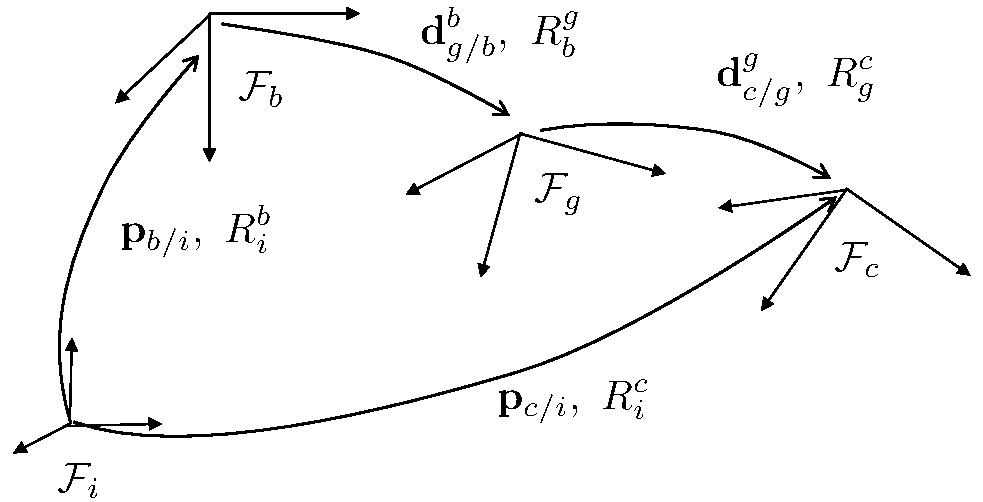
\includegraphics[width=\linewidth]{chap9_visual_servoing/figures/body_gimbal_camera}
	\caption{The relationship between the body frame, the gimbal frame, and the camera frame.}
	\label{fig:body_gimbal_camera}
\end{marginfigure}
The camera frame $\mathcal{F}_c = \{\ibf_c, \jbf_c, \kbf_c\}$ is defined so that $\ibf_c$ points to the right in the image, $\jbf_c$ points down, and $\kbf_c$ points along the optical axis.  The gimbal frame $\mathcal{F}_g = \{\ibf_g, \jbf_g, \kbf_g\}$ is defined so that $\ibf_g$ points along the optical axis, $\jbf_g$ points to the right in the image, and $\kbf_g$ points down in the image.  Therefore
\[
R_g^c = \begin{pmatrix}0 & 1 & 0 \\ 0 & 0 & 1 \\ 1 & 0 & 0 \end{pmatrix}.
\]

The gimbal frame $\mathcal{F}_g$ is obtained by first rotating about the body $z$-axis by the azimuth angle $\alpha$ to obtain the gimbal-1 frame, and then rotating about the gimbal-1 frame by the elevation angle $\beta$ to obtain the gimbal frame. Therefore
\begin{align*}
R_b^g &= R_{g1}^g R_b^{g1} \\
	  &= \begin{pmatrix} \cos\beta & 0 & \sin\beta \\ 0 & 1 & 0 \\ -\sin\beta & 0 & 1 \end{pmatrix} \begin{pmatrix} \cos\alpha & -\sin\alpha & 0 & \\ \sin\alpha & \cos\alpha & 0 \\ 0 & 0 & 1 \end{pmatrix} \\
	  &= \begin{pmatrix}
	  \cos\beta\cos\alpha & -\cos\beta\sin\alpha & \sin\beta \\
	  \sin\alpha & \cos\alpha & 0 \\
	  -\sin\beta\cos\alpha & \sin\beta\sin\alpha & \cos\beta
	  \end{pmatrix}.
\end{align*}

The follow theorem gives the most general result.
\begin{theorem}
	If the inertial position of the feature is moving with velocity $\vbf_{f/i}^i$, and suppose that the multirotor is moving with velocity $\vbf_{b/i}^i$ and angular velocity $\omegabf_{b/i}^b$, and that the gimbal is rotating with angular velocity $\omegabf_{g/b}^g$, then the pixel motion of the feature satisfies
	\begin{equation} \label{eq:optic_flow_full}
	\dot{\epsilonbf}_f =G_1(\epsilonbf_f, \lambda_f, t) (\vbf_{b/i}^i-\vbf_{f/i}^i)
	+ G_2(\epsilonbf_f, \lambda_f, t) \omegabf_{b/i}^b
	+ G_3(\epsilonbf_f, \lambda_f) \omegabf_{g/b}^g.
	\end{equation}
	where
	\begin{align*}
	G_1(\boldsymbol{\epsilon}_f, \lambda_f, t) & \defeq 	\lambda_f V(\boldsymbol{\epsilon}_f) R_g^c R_b^g(t) R_i^b(t) \\
	G_2(\epsilonbf_f, \lambda_f, t) & \defeq  \boldsymbol{\Omega}(\epsilonbf_f)R_g^c R_b^g(t) - \lambda_f V(\epsilonbf_f) R_g^c R_b^g(t) \ss{\dbf_{g/b}^b+R_g^b(t) \dbf_{c/g}^g} \\
	G_3(\epsilonbf_f, \lambda_f) & \defeq 	\boldsymbol{\Omega}(\epsilonbf_f) R_g^c - \lambda_f V(\epsilonbf_f) R_g^c \ss{\dbf_{c/g}^g}.
	\end{align*}
\end{theorem}
\begin{proof}
Using Figure~\ref{fig:body_gimbal_camera} we see that the inertial position of the camera frame, expressed in the inertial frame is given by
\begin{align}
\pbf_{c/i}^i &= \pbf_{b/i}^i + \dbf_{g/b}^i + \dbf_{c/g}^i \notag \\
&= \pbf_{b/i}^i + R_b^i\dbf_{g/b}^b + R_b^i R_g^b \dbf_{c/g}^g. \label{eq:pos_camera_inertial}
\end{align}
And that the rotation matrices satisfy
\[
R_i^c = R_g^c R_b^g R_i^b.
\]
Since the vectors are expressed in the inertial frame, we can differentiate with respect to time to obtain
\[
\mathbf{v}_{c/i}^i = \mathbf{v}_{b/i}^i + \dot{R}_b^i\mathbf{d}_{g/b}^b + R_b^i\dot{\mathbf{d}}_{g/b}^b 
+ \dot{R}_b^i R_g^b \mathbf{d}_{c/g}^g + R_b^i \dot{R}_g^b \mathbf{d}_{c/g}^g + R_b^i R_g^b \dot{\mathbf{d}}_{c/g}^g.
\]
Since the position of the gimbal is fixed in the body frame, we have $\dot{\mathbf{d}}_{g/b}^b=0$, and since the position of the camera is fixed in the gimbal frame we have that $\dot{\mathbf{d}}_{c/g}^g=0$.  From Equation~\eqref{eq:dR_dti} we have that $\dot{R}_b^i=R_b^i(\boldsymbol{\omega}_{b/i}^b)^\times$ and $\dot{R}_g^b = R_g^b (\boldsymbol{\omega}_{g/b}^g)^\times$.  Therefore we have 
\[
\mathbf{v}_{c/i}^i = \mathbf{v}_{b/i}^i + R_b^i(\boldsymbol{\omega}_{b/i}^b)^\times\mathbf{d}_{g/b}^b  
+ R_b^i(\boldsymbol{\omega}_{b/i}^b)^\times R_g^b \mathbf{d}_{c/g}^g + R_b^i R_g^b (\boldsymbol{\omega}_{g/b}^g)^\times \mathbf{d}_{c/g}^g,
\]
or expressed in the camera frame
\[
\mathbf{v}_{c/i}^c = R_g^c R_b^g R_i^b\mathbf{v}_{b/i}^i + R_g^c R_b^g(\boldsymbol{\omega}_{b/i}^b)^\times\mathbf{d}_{g/b}^b  
+ R_g^c R_b^g(\boldsymbol{\omega}_{b/i}^b)^\times R_g^b \mathbf{d}_{c/g}^g + R_g^c (\boldsymbol{\omega}_{g/b}^g)^\times \mathbf{d}_{c/g}^g.
\]
Using the fact that $\mathbf{a}^\times \mathbf{b} = - \mathbf{b}^\times \mathbf{a}$ we gives
\begin{align}
\mathbf{v}_{c/i}^c &= R_g^c R_b^g R_i^b \mathbf{v}_{b/i}^i - R_g^c R_b^g(\mathbf{d}_{g/b}^b)^\times \boldsymbol{\omega}_{b/i}^b  
- R_g^c R_b^g(R_g^b \mathbf{d}_{c/g}^g)^\times \boldsymbol{\omega}_{b/i}^b  - R_g^c (\mathbf{d}_{c/g}^g)^\times \boldsymbol{\omega}_{g/b}^g \notag \\
&= \left[R_g^c R_b^g R_i^b\right]\mathbf{v}_{b/i}^i - \left[ R_g^c R_b^g(\mathbf{d}_{g/b}^b+R_g^b \mathbf{d}_{c/g}^g)^\times \right] \boldsymbol{\omega}_{b/i}^b  
- \left[R_g^c (\mathbf{d}_{c/g}^g)^\times \right] \boldsymbol{\omega}_{g/b}^g. \label{eq:v_c_^c}
\end{align}

Also, since angular velocities add, we have 
\[
\boldsymbol{\omega}_{c/i}^c = \boldsymbol{\omega}_{c/g}^c + \boldsymbol{\omega}_{g/b}^c + \boldsymbol{\omega}_{b/i}^c.
\]
Assuming that the camera is stationary with respect to the gimbal, i.e., $\boldsymbol{\omega}_{c/g}^c=0$ gives
\begin{equation} \label{eq:omega_c^c}
\boldsymbol{\omega}_{c/i}^c = R_g^c \boldsymbol{\omega}_{g/b}^g + R_g^c R_b^g \boldsymbol{\omega}_{b/i}^b.	
\end{equation}

Using Equations~\eqref{eq:v_c_^c} and~\eqref{eq:omega_c^c} in Equation~\eqref{eq:optic_flow} gives the following expression for the pixel motion
\begin{multline} \label{eq:optic_flow_full_pre}
\dot{\boldsymbol{\epsilon}}_f = \lambda_f \left[V(\epsilonbf_f) R_g^c R_b^g R_i^b \right] (\vbf_{b/i}^i-\vbf_{f/i}^i) \\
+ \left[\boldsymbol{\Omega}(\boldsymbol{\epsilon}_f)R_g^c R_b^g - \lambda_f V(\boldsymbol{\epsilon}_f) R_g^c R_b^g (\dbf_{g/b}^b+R_g^b \dbf_{c/g}^g)^\times \right] \omegabf_{b/i}^b \\
+ \left[\boldsymbol{\Omega}(\epsilonbf_f) R_g^c - \lambda_f V(\epsilonbf_f) R_g^c (\dbf_{c/g}^g)^\times \right] \omegabf_{g/b}^g.
\end{multline}

\end{proof}

\begin{corollary}
	If the distance to the feature is large relative to the lengths $\dbf_{g/b}^b$ and $\dbf_{c/g}^g$, then the pixel motion is
	\[
	\dot{\epsilonbf}_f =G_1(\epsilonbf_f, \lambda_f, t) (\vbf_{b/i}^i-\vbf_{f/i}^i)
	+ G_2'(\epsilonbf_f, t) \omegabf_{b/i}^b
	+ G_3'(\epsilonbf_f) \omegabf_{g/b}^g.
	\]
	where
	\begin{align*}
	G_2'(\epsilonbf_f, t) & \defeq  \boldsymbol{\Omega}(\epsilonbf_f)R_g^c R_b^g(t)  \\
	G_3'(\epsilonbf_f, \lambda_f) & \defeq 	\boldsymbol{\Omega}(\epsilonbf_f) R_g^c.
	\end{align*}
\end{corollary}
\begin{proof}
	If the distance to the feature is large relative to the lengths $\dbf_{g/b}^b$ and $\dbf_{c/g}^g$ then 
	\begin{align*}
	\lambda_f\ss{\dbf_{g/b}^b + R_g^b\dbf_{c/g}^g} &\approx 0 \\
	\lambda_f \ss{\dbf_{c/g}^g} &\approx 0.
	\end{align*}
\end{proof}

\begin{corollary} \label{cor:visual_servoing_no_gimbal}
	If the camera is fixed in the body frame (no gimbal), and the distance to the feature is large relative to the lengths $\dbf_{c/b}^b$, then the pixel motion is
	\[
	\dot{\epsilonbf}_f = \lambda_f V(\epsilonbf_f)R_b^c R_i^b(t)(\vbf_{b/i}^i - \vbf_{f/i}^i) + \boldsymbol{\Omega}(\epsilonbf_f) R_b^c \omegabf_{b/i}^b.
	\]
\end{corollary}

\begin{lemma}
	The rank of the matrices $V(\epsilonbf_f)$ and $\boldsymbol{\Omega}(\epsilonbf_f)$ is two for all $\epsilonbf_f$.  If the gimbal is stationary, and $\lambda_z\neq\infty$ (feature depth of zero), then 
	\[
	\text{rank}(G_1) = \text{rank}(G_2) = \text{rank}(G_3) = 2.
	\]	
\end{lemma}
\begin{proof}
	From Equation~\eqref{eq:V(epsilon)} it is clear that $\text{rank}(V(\boldsymbol{\epsilon}_\ell))=2$ for any $\boldsymbol{\epsilon}_\ell$.  To show that $\Omega(\boldsymbol{\epsilon}_\ell)$ also has rank of two, note from Equation~\eqref{eq:Omega(epsilon)} that if $\epsilon_x=\epsilon_y=0$, then the rows of $\Omega(\boldsymbol{\epsilon}_\ell)$ are $(0, -1, 0)$ and $(1, 0, 0)$ which are linearly independent.  Now suppose that $\epsilon_y\neq 0$, then
	\[
	c_1\begin{pmatrix} \epsilon_x\epsilon_y \\ 1 + \epsilon_y^2 \end{pmatrix} + c_2 \begin{pmatrix} \epsilon_y \\ -\epsilon_x \end{pmatrix} = 0,
	\]
	implies that $c_2 = -c_1\epsilon_x$ and therefore $c_1(1 + \epsilon_x^2 + \epsilon_y^2)=0$, which implies that $c_1=c_2=0$, and therefore the first and last columns of $\Omega(\epsilonbf_f)$ are linearly independent.  A similar argument can be made for the case of $\epsilon_x\neq 0$.  Therefore $\text{rank}(\Omega(\epsilonbf_f))=2$ for any $\epsilonbf_f$.
	Since $R_a^b$ are rotation matrices, Sylvester's inequality and assumption A3 imply that $\text{rank}(G_1)=2$.  

	The matrix $G_2$ can be written as
	\[
	G_2 = \begin{pmatrix} \boldsymbol{\Omega}R_g^cR_b^g, & \lambda_f V R_g^cR_b^g \end{pmatrix} \begin{pmatrix} I_3 \\ -(\mathbf{d}_{g/b}^b+R_g^b(t) \mathbf{d}_{c/g}^g)^\times \end{pmatrix},
	\]
	where the first matrix is rank two following an argument similar to the previous paragraph, and the second matrix is clearly rank 3.  Therefore $\text{rank}(G_2)=2$ by Sylvester's inequality.
 	A similar argument can be made for $G_3$.
\end{proof}

%-----------------------------------------------------------
\section{The Body-Level Frame}
\label{sec:body_level_frame}

\begin{marginfigure}
	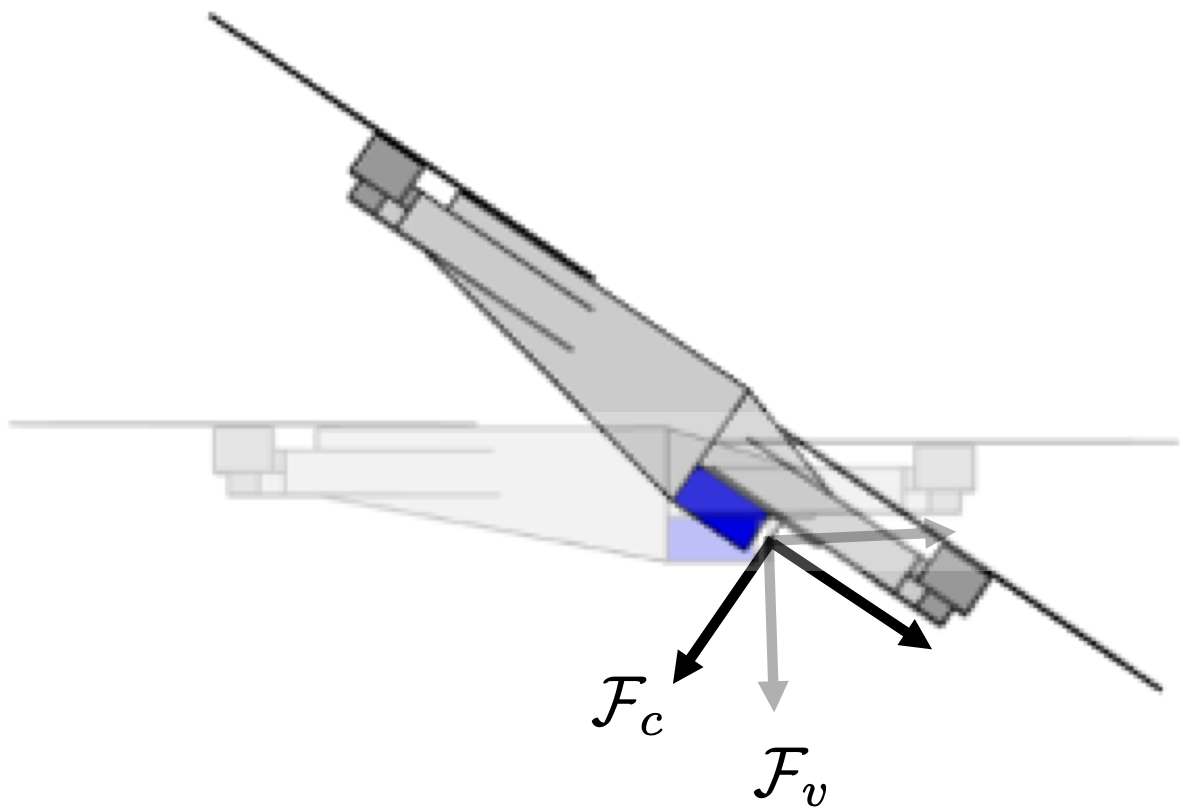
\includegraphics[width=\linewidth]{chap9_visual_servoing/figures/body_level_frame}
	\caption{The body-level frame results by rotating the body frame by the negative roll and pitch angles.  The only rotation in the body-level frame is due to yaw.}
	\label{fig:body_level_frame}
\end{marginfigure}

The landing and target following problem will be cast in the body-level frame.  The basic idea is that the body-level frame is the un-rolled and un-pitched body frame.  The heading direction for the body frame and the body-level frame will be identical, but the $z$-axis of the body level frame will always point down along the gravity vector.
Letting $\ell$ denote the body-level frame, we have that
\[
R_b^i = R_\ell^i R_b^\ell,
\]
or 
\[
R_\ell^i =  R_b^i (R_b^\ell)^\top.
\]
To make things concrete, if $\phi$, $\theta$, and $\psi$ are the roll, pitch, and yaw Euler angles, then 
\begin{align*}
R_b^i &= R_z(\psi) R_y(\theta) R_x(\phi) \\
&\defeq \begin{pmatrix} \cos\psi & -\sin\psi & 0 \\ \sin\psi & \cos\psi & 0 \\ 0 & 0 & 1 \end{pmatrix}
\begin{pmatrix} \cos\theta & 0 & \sin\theta \\ 0 & 1 & 0 \\ -\sin\theta & 0 & \cos\theta \end{pmatrix}
\begin{pmatrix} 1 & 0 & 0 \\ 0 & \cos\phi & -\sin\phi \\ 0 & \sin\phi & \cos\phi \end{pmatrix}.
\end{align*}
In this case $R_\ell^i = R_z(\psi)$ and $R_b^\ell = R_y(\theta)R_x(\phi)$.

Since the origin of the body-level frame is coincident with the origin of the body frame, we have that
\begin{align*}
\mathbf{p}_{\ell/i} &= \mathbf{p}_{b/i} \\	
\mathbf{v}_{\ell/i} &= \mathbf{v}_{b/i}.
\end{align*}

\begin{lemma} \label{lem:pixels_in_level_frame}
	The normalized pixel coordinates in the camera frame $\bar{\epsilonbf}_f^c$, and the scaling factor $\lambda_f^c$ are transformed to the level frame as 
	\begin{align*}
	\bar{\epsilonbf}_f^\ell &= \frac{R_b^\ell R_c^b \bar{\epsilonbf}_f^c}{\ebf_3^\top R_b^\ell R_c^b \bar{\epsilonbf}_f^c} \\
	\lambda_f^\ell &= \lambda_f^c \ebf_3^\top R_b^\ell R_c^b \bar{\epsilonbf}_f^c,
	\end{align*}
	where 
	\[
	\lambda_f^\ell \bar{\epsilonbf}_f^\ell = \pbf_{f/\ell}^\ell.
	\]
\end{lemma}
\begin{proof}
	The normalized pixel coordinates in the camera frame $\bar{\epsilonbf}_f^c$ can be transformed to the level frame as
	\[
	\epsilonbf_f^\ell = R_b^\ell R_c^b\bar{\epsilonbf}_f^c,
	\]
	but in this case the last element of $\epsilonbf_f^\ell$ will not necessarily be equal to unity.  Therefore, to obtain normalized coordinates we use
	\[
	\bar{\epsilonbf}_f^\ell = \frac{R_b^\ell R_c^b\bar{\epsilonbf}_f^c}{\ebf_3^\top R_b^\ell R_c^b\bar{\epsilonbf}_f^c}.
	\]
	Noting that
	\begin{align*}
	\lambda_f^\ell \bar{\epsilonbf}_f^\ell 
		&= \lambda_f^\ell \left(\frac{R_b^\ell R_c^b\bar{\epsilonbf}_f^c}{\ebf_3^\top R_b^\ell R_c^b\bar{\epsilonbf}_f^c} \right) \\
		&= \pbf_{f/\ell}^\ell \\
		&= R_b^\ell R_c^b \pbf_{f/c}^c \\
		&= \lambda_f^c R_b^\ell R_c^b \bar{\epsilonbf}_f^c
	\end{align*}
	which implies that
	\[
	\frac{\lambda_f^\ell}{\ebf_3^\top R_b^\ell R_c^b \bar{\epsilonbf}_f^c}(R_b^\ell R_c^b \bar{\epsilonbf}_f^c) = \lambda_f^c R_b^\ell R_c^b \bar{\epsilonbf}_f^c
	\]
	which gives the results.
\end{proof}

The pixel motion in the body-level frame becomes particularly simply.
\begin{lemma} \label{lem:visual_servoing_multirotor}
	Let $\vbf_{b/f}^i$ be the velocity of the body relative to the feature, and let $\omegabf_{\ell/i}^\ell =\omegabf_{\ell/i}^i = (0, 0, \omega_z)^\top$ be the angular velocity of the level frame,
	then the pixel motion in the body-level frame virtual camera is given by
	\[
	\dot{\epsilonbf}_f^\ell = G_f \nubf^\ell,
	\]
	where
	\begin{align*}
	\nubf^\ell &= (\vbf_{b/f}^{i\top}, ~\omega_z)^\top \\
	G_f &= \begin{pmatrix}
			\lambda_f^\ell V(\epsilonbf_f^\ell) R_i^\ell, & \boldsymbol{\Omega}(\epsilonbf_f^\ell)\ebf_3
		   \end{pmatrix}.
	\end{align*}
	
\end{lemma}
\begin{proof}
	From Corollary~\ref{cor:visual_servoing_no_gimbal}, replacing the body frame with the body-level frame, we have
		\[
		\dot{\epsilonbf}_f^\ell = \lambda_f V(\epsilonbf_f^\ell)R_\ell^c R_i^\ell(t)(\vbf_{\ell/i}^i - \vbf_{f/i}^i) + \boldsymbol{\Omega}(\epsilonbf_f^\ell) R_\ell^c \omegabf_{\ell/i}^\ell.
		\]
		Noting that the virtual camera frame and the body-level frame are identical, i.e., $R_\ell^c=I$ gives
		\[
		\dot{\epsilonbf}_f^\ell = \lambda_f V(\epsilonbf_f^\ell) R_i^\ell(t)(\vbf_{\ell/i}^i - \vbf_{f/i}^i) + \boldsymbol{\Omega}(\epsilonbf_f^\ell) \omegabf_{\ell/i}^\ell.
		\]
		The result follows by noting that 
		\begin{align*}
		\boldsymbol{\Omega}(\epsilonbf_f^\ell) \omegabf_{\ell/i}^\ell 
			&= \boldsymbol{\Omega}(\epsilonbf_f^\ell) \begin{pmatrix} 0 \\ 0 \\ \omega_z \end{pmatrix} \\
			&= \boldsymbol{\Omega}(\epsilonbf_f^\ell)\ebf_3 \omega_z.
		\end{align*}		
\end{proof}

%----------------------------------------------------------------
\section{Landing and target following using visual servoing}

This section describes how Lemma~\ref{lem:visual_servoing_multirotor} can be used to design algorithms for landing a multirotor on a moving target, and for following a moving target.

The basic idea is to maneuver the multirotor so that a set of feature points move to specified locations in the image plane.  Let 
\begin{equation}\label{eq:visual_servoing_sbf}
\sbf \defeq \begin{pmatrix}
\epsilonbf_{f_1}^\ell \\
\epsilonbf_{f_2}^\ell \\
\vdots \\
\epsilonbf_{f_m}^\ell
\end{pmatrix},
\end{equation}
be a set of feature point and let 
\begin{equation}\label{eq:visual_servoing_sbf_d}
\sbf_d(t) = \begin{pmatrix}
\epsilonbf_{d_1}^{\ell}(t) \\
\epsilonbf_{d_2}^{\ell}(t) \\
\vdots \\
\epsilonbf_{d_m}^{\ell}(t)
\end{pmatrix},
\end{equation}
be the set of time-varying desired feature locations, and let $\tilde{\sbf} \defeq \sbf - \sbf_d$.  Differentiating $\tilde{\sbf}$ gives
\begin{align*}
\dot{\sbf} &= \dot{\sbf} - \dot{\sbf}_d \\
		   &= \begin{pmatrix} G_{f_1} \\ \dots \\ G_{f_m} \end{pmatrix} \nubf^\ell - \dot{\sbf}_d \\
		   &= G_m \nubf^\ell - \dot{\sbf}_d,
\end{align*}
where 
\[
G_m \defeq \begin{pmatrix} G_{f_1} \\ \dots \\ G_{f_m} \end{pmatrix}.
\]

\begin{lemma} \label{lem:G_rank_4}
	Let $\{\epsilonbf_{f_1}, \dots, \epsilonbf_{f_m}\}$ be a set of 2D normalized pixel locations, where at least two points are not scaled version of each other, i.e., there exists $i\neq j$, such that $\epsilonbf_{f_j} \neq \mu\epsilonbf_{f_j}$ for any $\mu$, then $\text{rank}(G_m)=4$.
\end{lemma}
\begin{proof}
	Without loss of generality, let $\epsilonbf_{f_1}$ and $\epsilonbf_{f_2}$ be two features points that are not scaled version of each other.  Consider the matrix 
	\[
	\hat{G} = \begin{pmatrix} G_{f_1} \\ G_{f_2} \end{pmatrix}.
	\]
	We will show that $\text{rank}(\hat{G})=4$, which implies that $\text{rank}(G_m)=4$, since adding additional rows cannot decrease the rank. 
	Toward that end, note that 
	\begin{align*}
	G_{f_i} &= \begin{pmatrix} \lambda_{f_i} V(\epsilonbf_{f_i})R_\ell^i, & \boldsymbol{\Omega}(\epsilonbf_{f_i})\ebf_3
			\end{pmatrix} \\
			&= \begin{pmatrix} \lambda_{f_i} \begin{pmatrix} -I_{2\times 2}, & \epsilonbf_{f_i}\end{pmatrix}\begin{pmatrix} R_\psi & \mathbf{0}_{2\times 1} \\ \mathbf{0}_{1\times 2} & 1 \end{pmatrix}, & J\epsilonbf_{f_i} \end{pmatrix}\\
			&= \begin{pmatrix} -\lambda_{f_i} R_\psi, & \lambda_{f_i} \epsilonbf_{f_i}, & J\epsilonbf_{f_i} \end{pmatrix},
	\end{align*}
	where $R_\psi\in SO(2)$ is the $2\times 2$ rotation matrix in the N-E plane, and $J=\begin{pmatrix} 0 & 1 \\ -1 & 0 \end{pmatrix}$ corresponds to a rotation in the image plane by $-\pi/2$.  
	Therefore
	\begin{align*}
	\hat{G} &= \begin{pmatrix} -\lambda_{f_1} R_\psi, & \lambda_{f_1} \epsilonbf_{f_1}, & J\epsilonbf_{f_1} \\ -\lambda_{f_2} R_\psi, & \lambda_{f_2} \epsilonbf_{f_2}, & J\epsilonbf_{f_2} \end{pmatrix} \\
	&= \begin{pmatrix} -\lambda_{f_1} I_{2\times 2}, & \lambda_{f_1} \epsilonbf_{f_1}, & J\epsilonbf_{f_1} \\ -\lambda_{f_2} I_{2\times 2}, & \lambda_{f_2} \epsilonbf_{f_2}, & J\epsilonbf_{f_2} \end{pmatrix} \begin{pmatrix}R_\psi & \mathbf{0}_{2\times 2} \\ \mathbf{0}_{2\times 2} & I_{2\times 2}\end{pmatrix} \\
	&= \begin{pmatrix} -\lambda_{f_1} I_{2\times 2}, & H(\lambda_{f_1}, \epsilonbf_{f_1}) \\ -\lambda_{f_2} I_{2\times 2}, & H(\lambda_{f_2}, \epsilonbf_{f_2}) \end{pmatrix} \begin{pmatrix}R_\psi & \mathbf{0}_{2\times 2} \\ \mathbf{0}_{2\times 2} & I_{2\times 2}\end{pmatrix},	
	\end{align*}
	where 
	\[
	H(\lambda, \epsilonbf) \defeq \begin{pmatrix} \lambda \epsilonbf, & J\epsilonbf \end{pmatrix}.
	\]
	Therefore $\text{rank}(\hat{G})=4$ if 
	\[
	\det{\begin{pmatrix} -\lambda_{f_1} I_{2\times 2}, & H(\lambda_{f_1}, \epsilonbf_{f_1}) \\ -\lambda_{f_2} I_{2\times 2}, & H(\lambda_{f_2}, \epsilonbf_{f_2}) \end{pmatrix}} \neq 0.
	\]
	Using the Schur identity 
	\[
	\det{\begin{pmatrix} A & B \\ C & D \end{pmatrix}} = \det{A}\det{(D-CA^{-1}B)}
	\]
	we get that
	\begin{align*}
	\det{\begin{pmatrix} -\lambda_{f_1} I_{2\times 2}, & H(\lambda_{f_1}, \epsilonbf_{f_1}) \\ -\lambda_{f_2} I_{2\times 2}, & H(\lambda_{f_2} \epsilonbf_{f_2}) \end{pmatrix}}
		&= -\lambda_{f_1} \det{\left(H(\lambda_{f_2},\epsilonbf_{f_2}) - \frac{\lambda_{f_2}}{\lambda_{f_1}}H(\lambda_{f_1},\epsilonbf_{f_1})\right)} \\
		&= -\lambda_{f_1} \det{\begin{pmatrix}\lambda_{f_2}\epsilon_{2x}, & \epsilon_{2y} \\ \lambda_{f_2}\epsilon_{2y}, & -\epsilon_{2x} \end{pmatrix}-\frac{\lambda_{f_2}}{\lambda_{f_1}}\begin{pmatrix}\lambda_{f_1}\epsilon_{1x}, & \epsilon_{1y} \\ \lambda_{f_1}\epsilon_{1y}, & -\epsilon_{1x}\end{pmatrix}} \\
		&= -\lambda_{f_1} \det{\begin{pmatrix}\lambda_{f_2}(\epsilon_{2x}-\epsilon_{1x}), & \epsilon_{2y}-\frac{\lambda_{f_2}}{\lambda_{f_1}}\epsilon_{1y} \\ \lambda_{f_2}(\epsilon_{2y}-\epsilon_{1y}), & \epsilon_{2x}-\frac{\lambda_{f_2}}{\lambda_{f_1}}\epsilon_{1x}\end{pmatrix}} \\
		&=-\lambda_{f_2}\left((\epsilon_{2x}-\epsilon_{1x})(\lambda_{f_2}\epsilon_{1x}-\lambda_{f_1}\epsilon_{2x}) -(\epsilon_{2y}-\epsilon_{1y})(\lambda_{f_1}\epsilon_{2y}-\lambda_{f_2}\epsilon_{1y}) \right) \\
		&= -\lambda_{f_2}\begin{pmatrix} \lambda_{f_1} & \lambda_{f_2}\end{pmatrix}^\top \begin{pmatrix} -\epsilon_{2x} & \epsilon_{2y} \\ \epsilon_{1x} & -\epsilon_{1y} \end{pmatrix}(\epsilonbf_{f_2}-\epsilonbf_{f_1}),
	\end{align*}
	which requires that both $\epsilonbf_{f_2}\neq\epsilonbf_{f_1}$ and that $E=\begin{pmatrix}-\epsilon_{2x} & \epsilon_{2y} \\ \epsilon_{1x} & -\epsilon_{1y} \end{pmatrix}$ is full rank.  But $E$ loses rank when
	\[
	\det{\begin{pmatrix}-\epsilon_{2x} & \epsilon_{2y} \\ \epsilon_{1x} & -\epsilon_{1y} \end{pmatrix}} 
		= \epsilon_{2x}\epsilon_{1y}-\epsilon_{1x}\epsilon_{2y}
		= \epsilonbf_{f_1}^\top J \epsilonbf_{f_2} = 0.
	\]
	Since $J$ represents a rotation in the image of $\pi/2$, $E$ loses rank only when $\epsilonbf_{f_1}=\mu\epsilonbf_{f_2}$ for some $\mu$.
\end{proof}

We can now state the main result for visual servoing control.
\begin{theorem}
	Let $\sbf$ and $\sbf_d(t)$ be defined as in Equations~\eqref{eq:visual_servoing_sbf} and~\eqref{eq:visual_servoing_sbf_d}, with $m=2$ feature points that are not scaled versions of each other, if the desired body velocity and desired heading vector are given by
	\begin{align*}
	\vbf_{d/i}^i &= \begin{pmatrix} I_{3\times 3}, 0_{3\times 1} \end{pmatrix} \nubf^\ell \\
	\sbf_{\psi_d} &= R_\ell^i \ebf_1,
	\end{align*}
	where $R_\ell^i$ satisfies
	\[
	\dot{R}_\ell^i = R_\ell^i \ss{ \begin{pmatrix} 0_{3\times 3}, \ebf_3 \end{pmatrix}\nubf^\ell},
	\]
	where
	\begin{equation}\label{eq:visual_servoing_nubf}
	\nubf^\ell = G_2^{-1}\left(\dot{\sbf}_d - K \tilde{\sbf}\right),
	\end{equation}
	where $K=K^\top>0$ is a positive definite gain matrix, then 
	\[
	\tilde{\sbf}(t) \to 0.
	\]
\end{theorem}
\begin{proof}
	Defining the Lyapunov function $V = \frac{1}{2}\norm{\tilde{s}}$ and differentiating gives
	\begin{align*}
	\dot{V} &= \tilde{\sbf}\top\dot{\tilde{\sbf}} \\
			&= G_2\nubf^\ell - \dot{\sbf}_d.
	\end{align*}
	Since the feature points are not co-linear, $G_2$ is invertible by Lemma~\ref{lem:G_rank_4}.  
	Selecting $\nubf^\ell$ according to Equation~\eqref{eq:visual_servoing_nubf}
	gives $\dot{V} = -\tilde{\sbf}^\top K \tilde{\sbf}$ from which we conclude that $\tilde{\sbf}\to 0$.
	Since $\nubf^\ell = (\vbf_{b/i}^{i\top}, \omega_z)^\top$ we have that
	\begin{align*}
	\vbf_{b/i}^i &= \begin{pmatrix} I, 0 \end{pmatrix} \nubf^\ell \\
	\omegabf_{\ell/i}^i &= \begin{pmatrix} 0_{3\times 3}, \ebf_3 \end{pmatrix}\nubf^\ell.
	\end{align*}
    The theorem is completed by noting that 
    \[
    \sbf_{\psi} = \begin{pmatrix}\cos\psi \\ \sin\psi \\ 0 \end{pmatrix} = \begin{pmatrix} \cos\psi & -\sin\psi & 0 \\ \sin\psi & \cos\psi & 0 \\ 0 & 0 & 1 \end{pmatrix}\ebf_1 = R_\ell^i \ebf_1.
    \]
\end{proof}

If we have more than two features in the image plane, then we have the following corollary.
\begin{corollary}
	Let $\sbf$ and $\sbf_d(t)$ be defined as in Equations~\eqref{eq:visual_servoing_sbf} and~\eqref{eq:visual_servoing_sbf_d}, with $m>2$ feature points, where at least two points are not scaled versions of each other.  If the desired body velocity and desired heading vector are given by
	\begin{align*}
	\vbf_{d/i}^i &= \begin{pmatrix} I_{3\times 3}, 0_{3\times 1} \end{pmatrix} \nubf^\ell \\
	\sbf_{\psi_d} &= R_\ell^i \ebf_1,
	\end{align*}
	where $R_\ell^i$ satisfies
	\[
	\dot{R}_\ell^i = R_\ell^i \ss{ \begin{pmatrix} 0_{3\times 3}, \ebf_3 \end{pmatrix}\nubf^\ell},
	\]
	where
	\[
	\nubf^\ell = G_2^{\dagger}\left(\dot{\sbf}_d - K \tilde{\sbf}\right),
	\]
	where $K=K^\top>0$ is a positive definite gain matrix and $A^\dagger$ is the pseudo-inverse of $A$, then 
	\[
	\lim_{t\to\infty}\norm{\tilde{s}(t)}
	\]
	is minimized.
\end{corollary}

\section{Multiple View Geometry-Transformations of a plane}
\rwbcomment{Add the stuff about affine homography transformations to show how to manipulate the desired pixels $\sbf_d$.  Use a discussion similar to the following pages from Multiple View Geometry.}
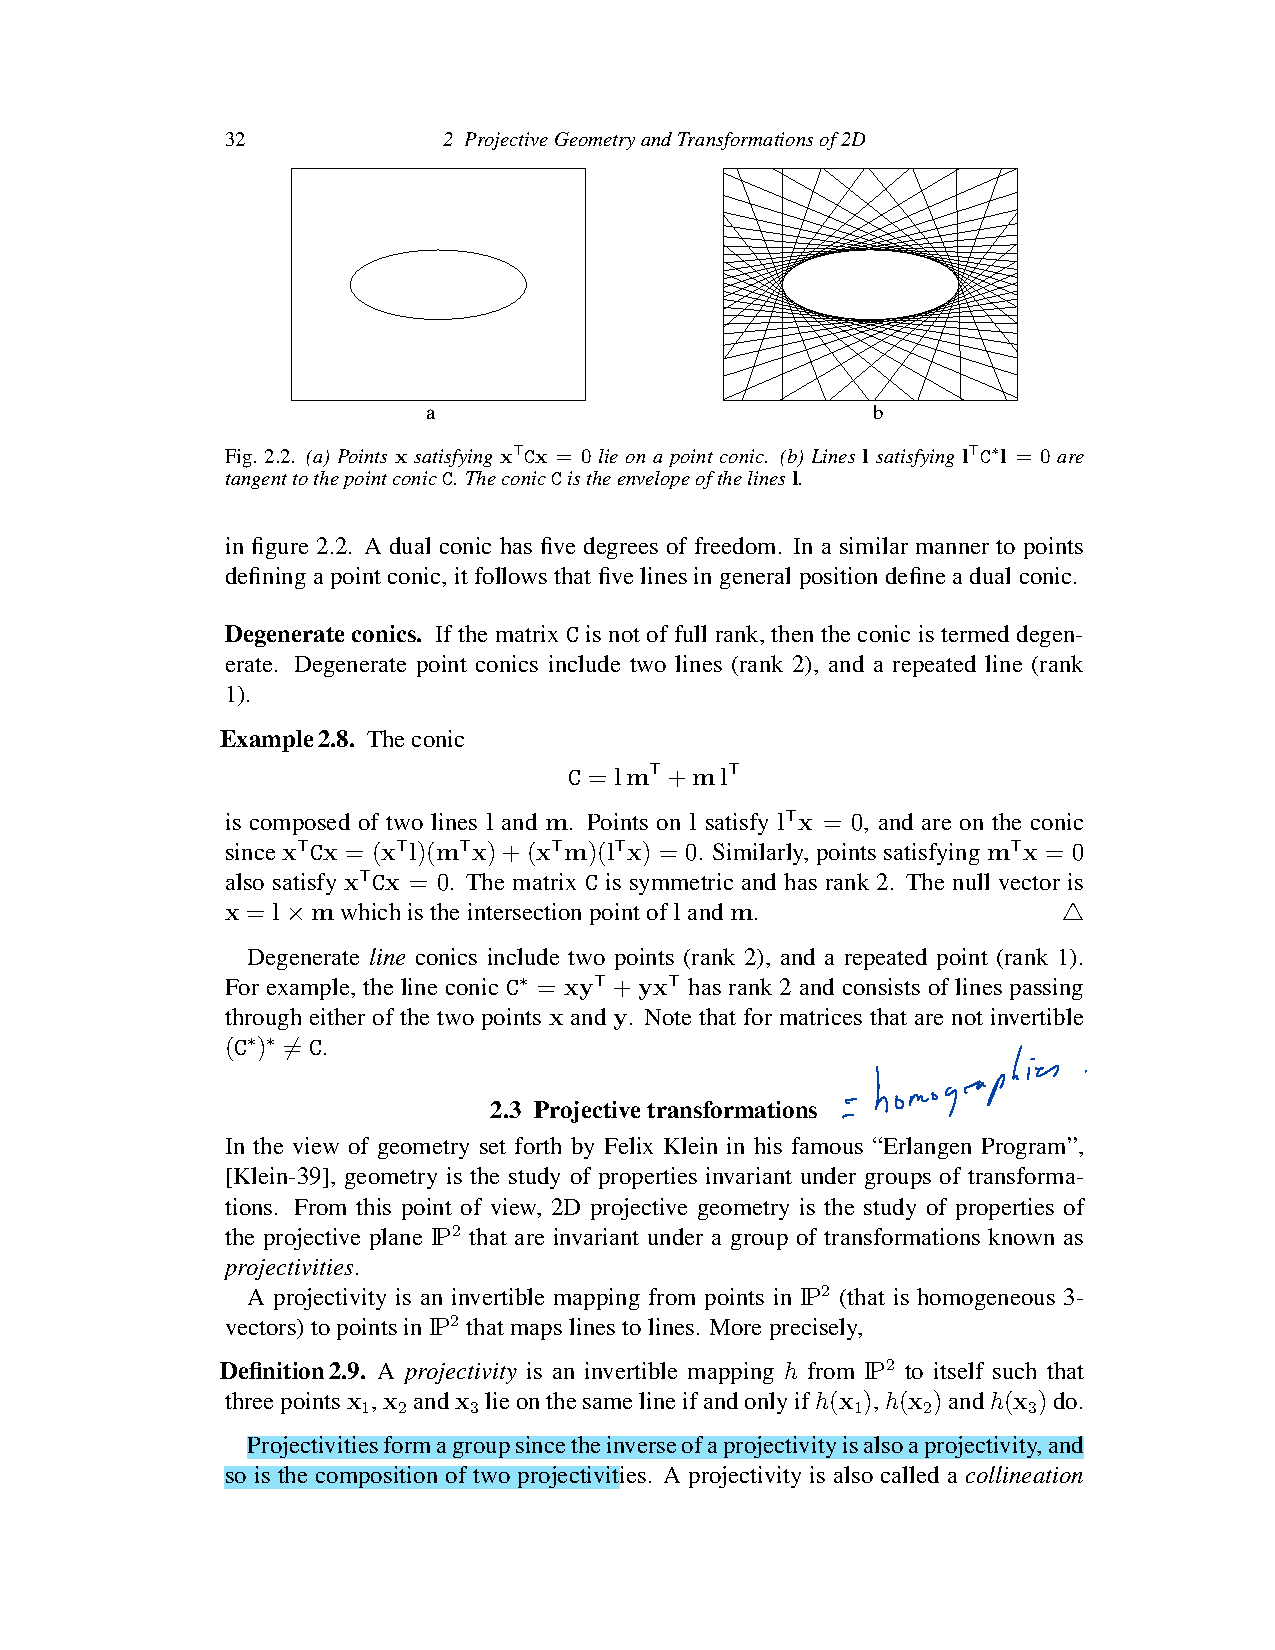
\includepdf[pages=-,scale=0.8,pagecommand={}]{chap9_visual_servoing/papers/HartleyZisserman00_homography2.pdf}

\section{Visual Servo Control Part I: Basic Approaches, RAM, 2006}
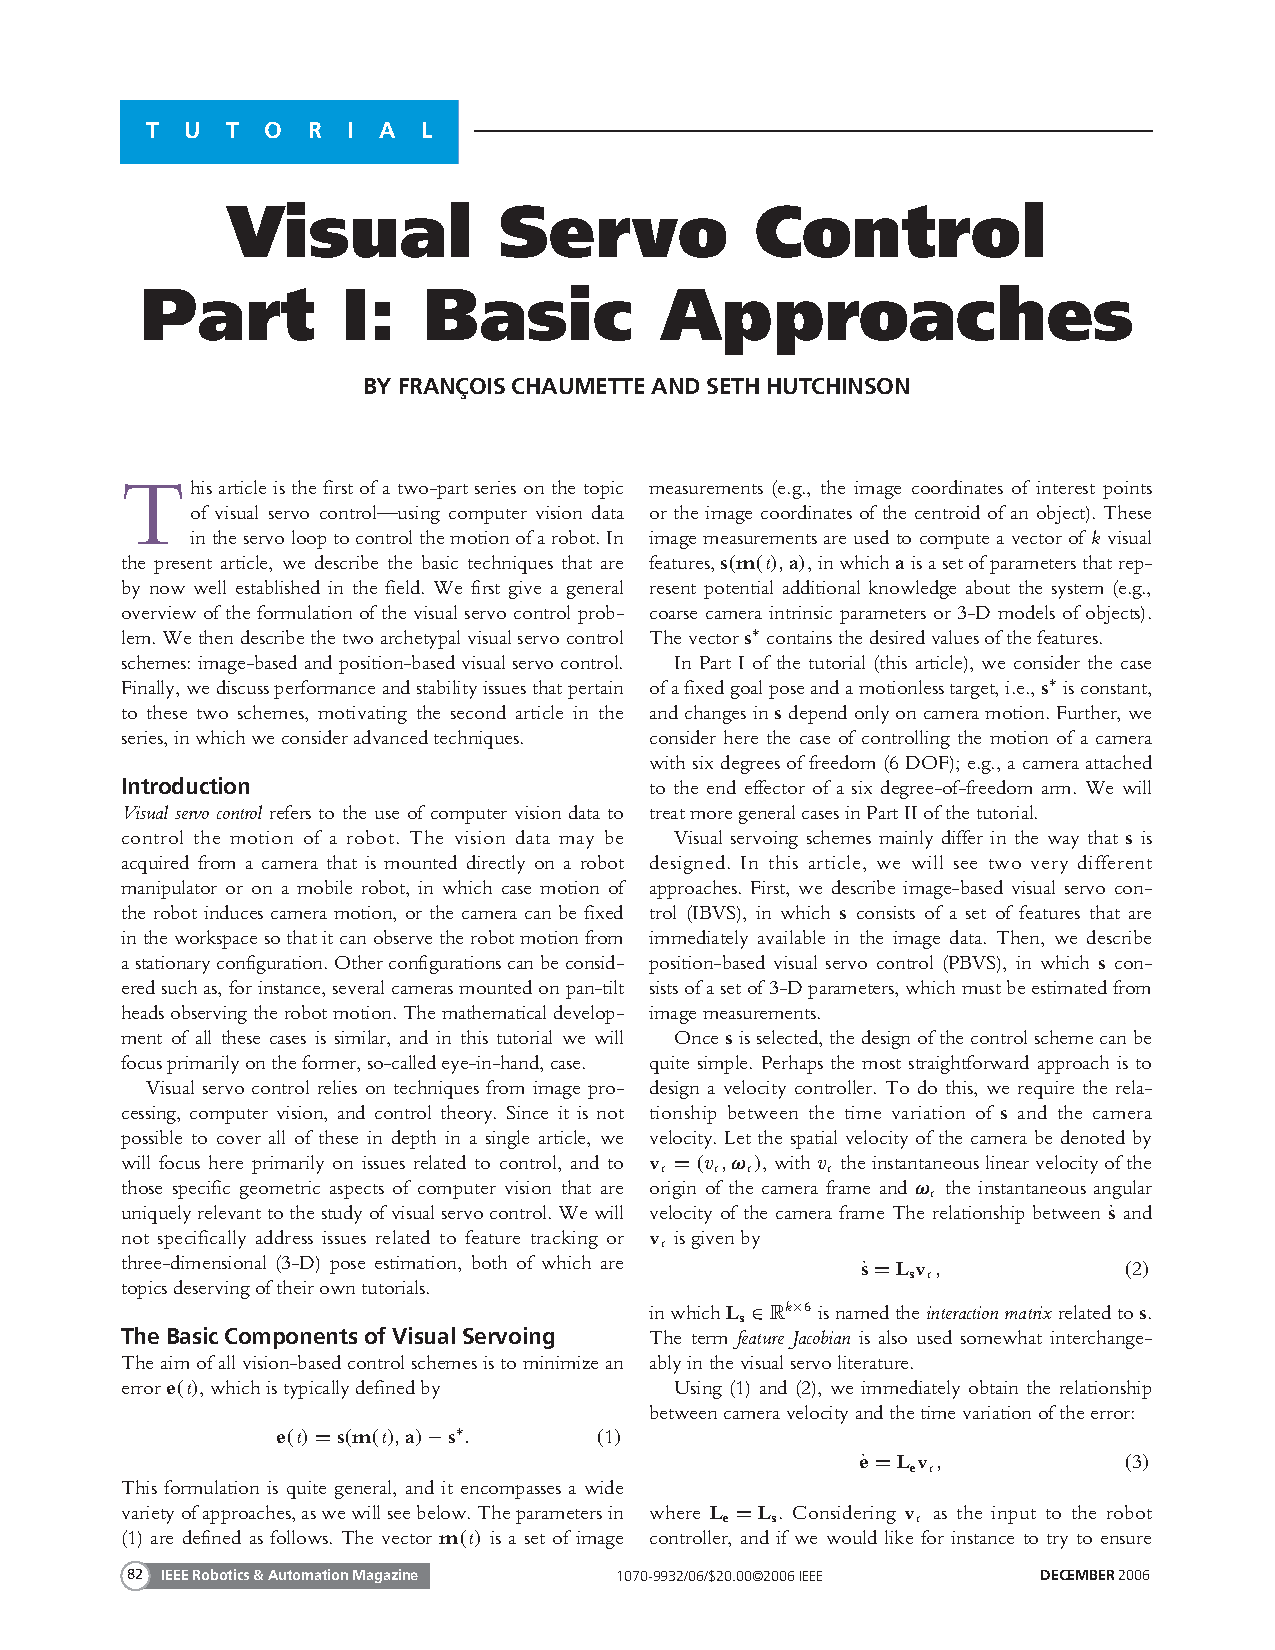
\includepdf[pages=-,scale=.8,pagecommand={}]{chap9_visual_servoing/papers/ChaumetteHutchinson06.pdf}

\section{Visual Servo Control Part II: Advanced Approaches, RAM, 2007}
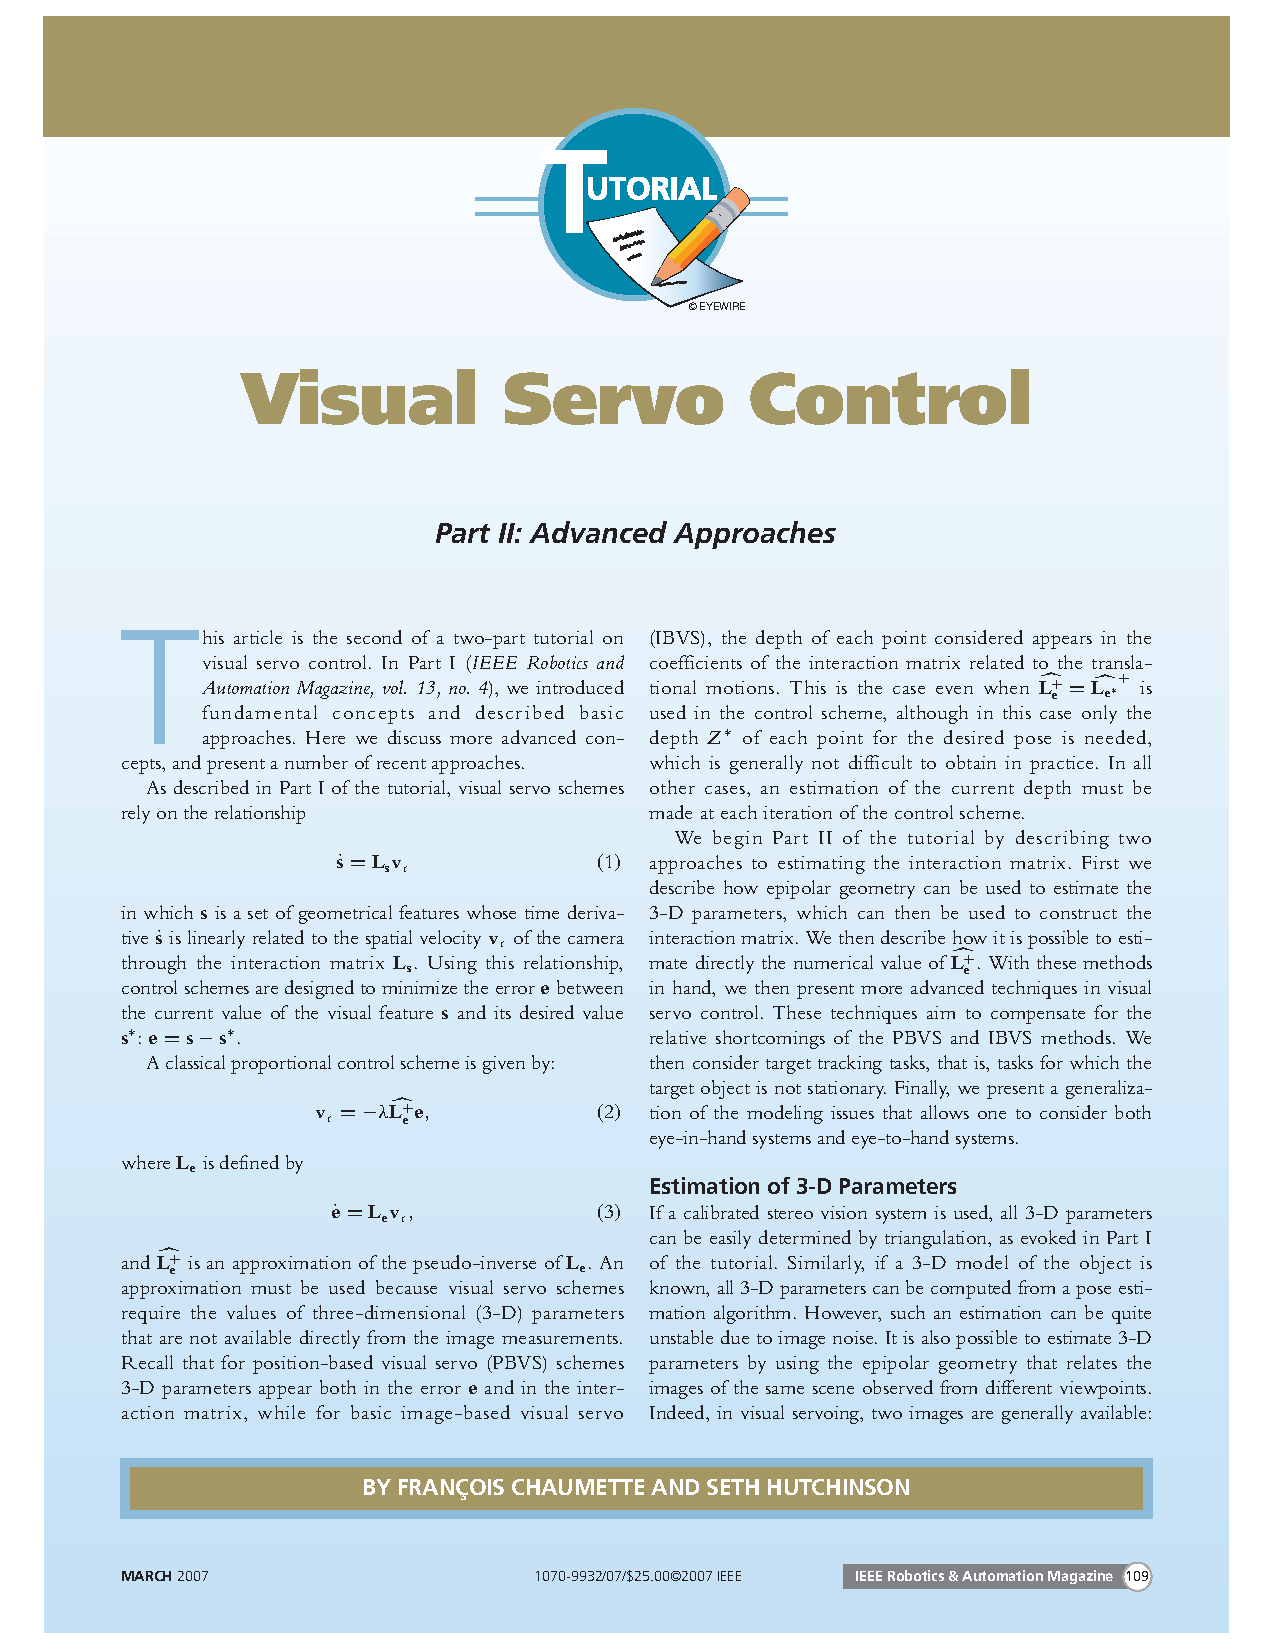
\includepdf[pages=-,scale=.8,pagecommand={}]{chap9_visual_servoing/papers/ChaumetteHutchinson07.pdf}

\section{Autonomous Landing of a VTOL UAV on a Moving Platform Using Image-based Visual Servoing, ICRA, 2012}
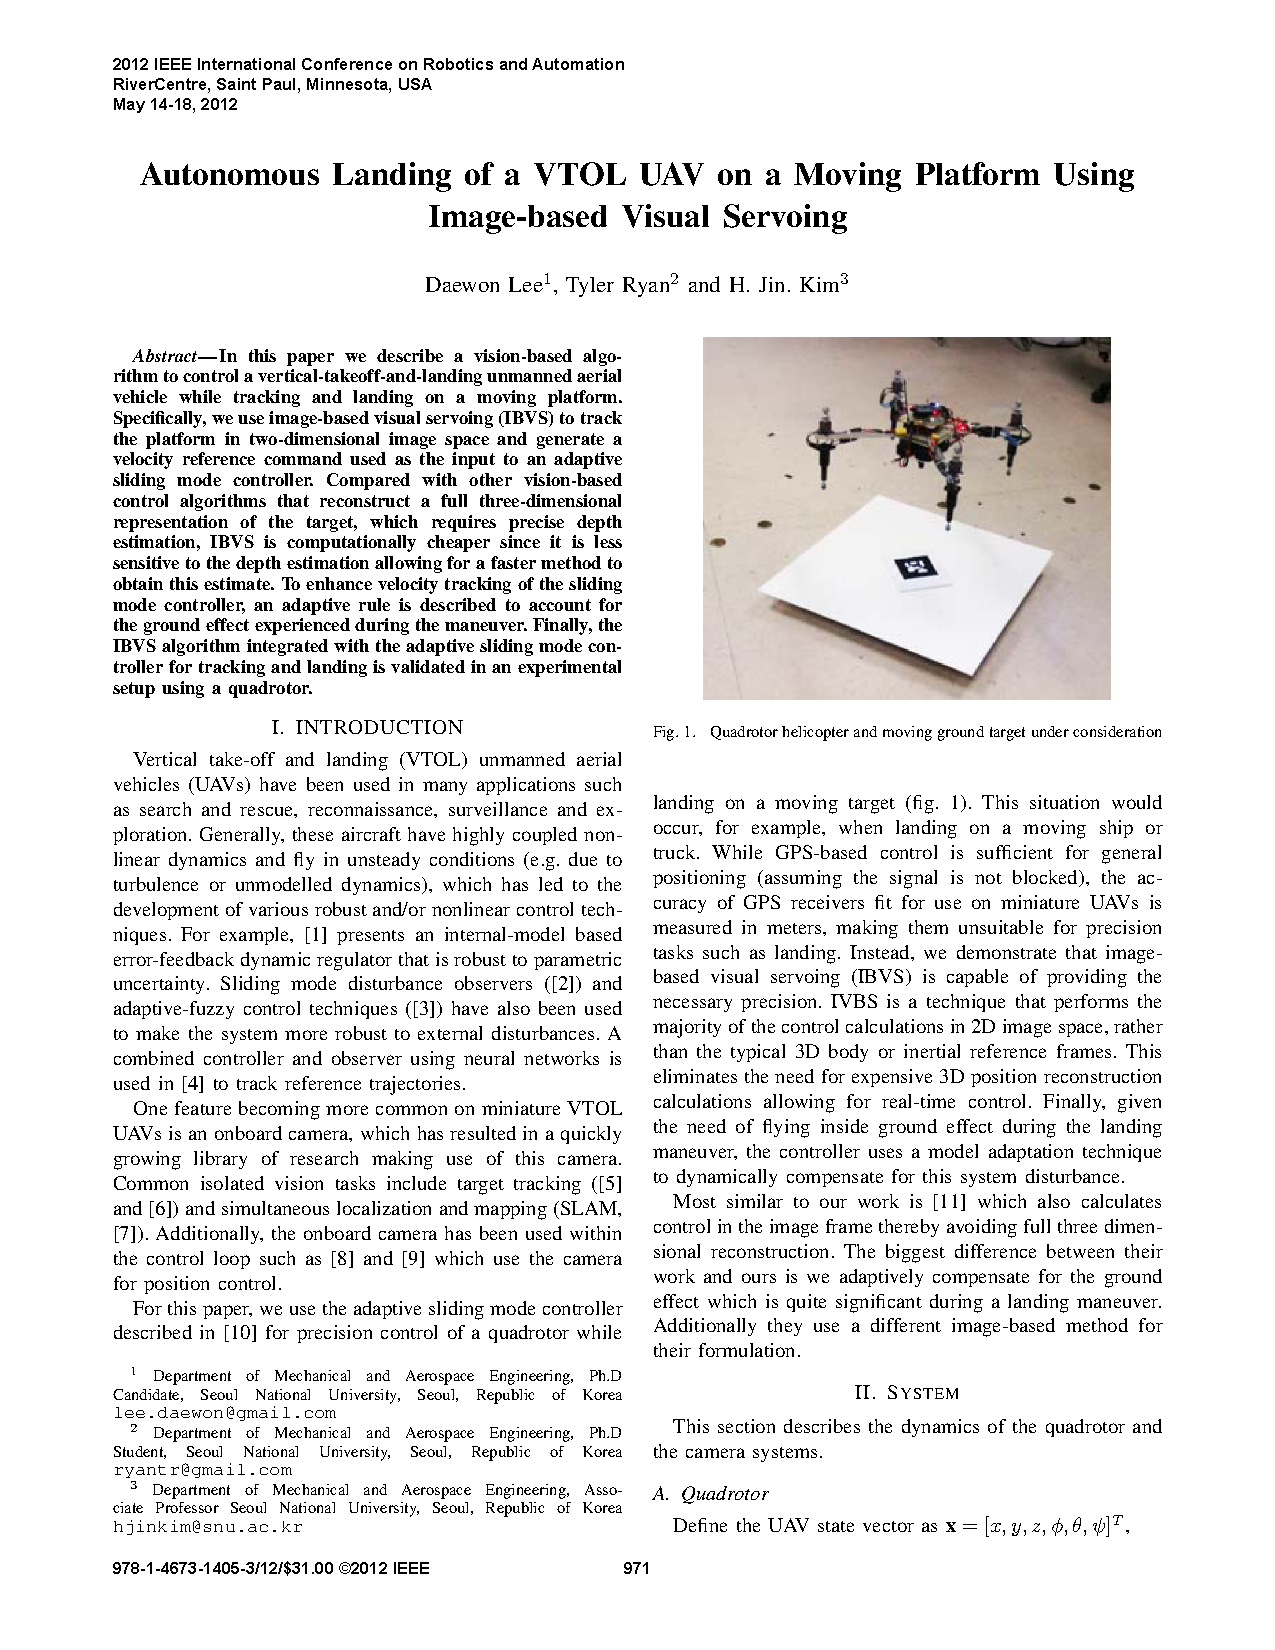
\includepdf[pages=-,scale=.8,pagecommand={}]{chap9_visual_servoing/papers/LeeRyanKim12.pdf}



%----------------------------------------------------------------------------
\section{Using visual servoing to point the gimbal at a target}
\rwbcomment{Do something similar to the paper below.}
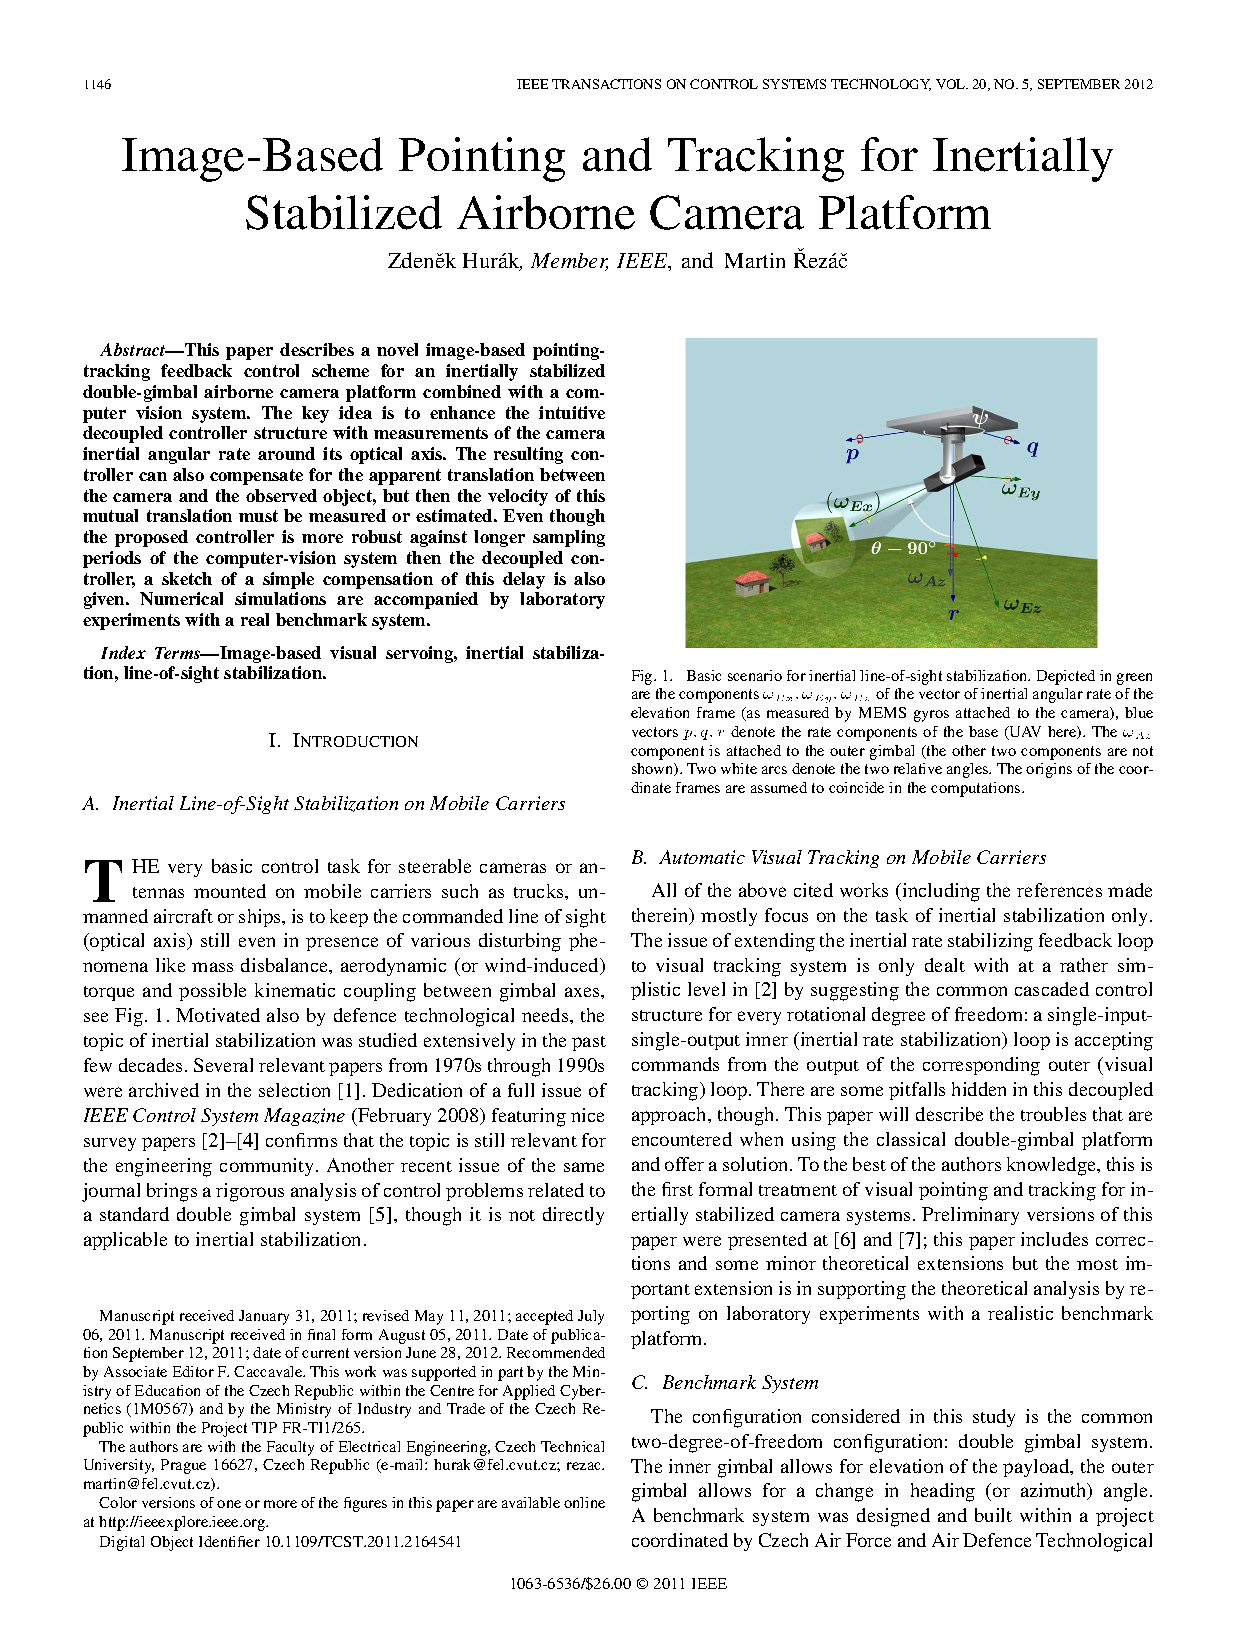
\includepdf[pages=-,scale=.8,pagecommand={}]{chap9_visual_servoing/papers/HurakRezac12.pdf}

%%----------------------------------
%\section{Collision Avoidance}
%\label{sec:collision_avoidance}
%
%\section{Vision-Based Local-Level Frame Mapping and Planning in Spherical Coordinates for Miniature Air Vehicles, TCST, 2013}
%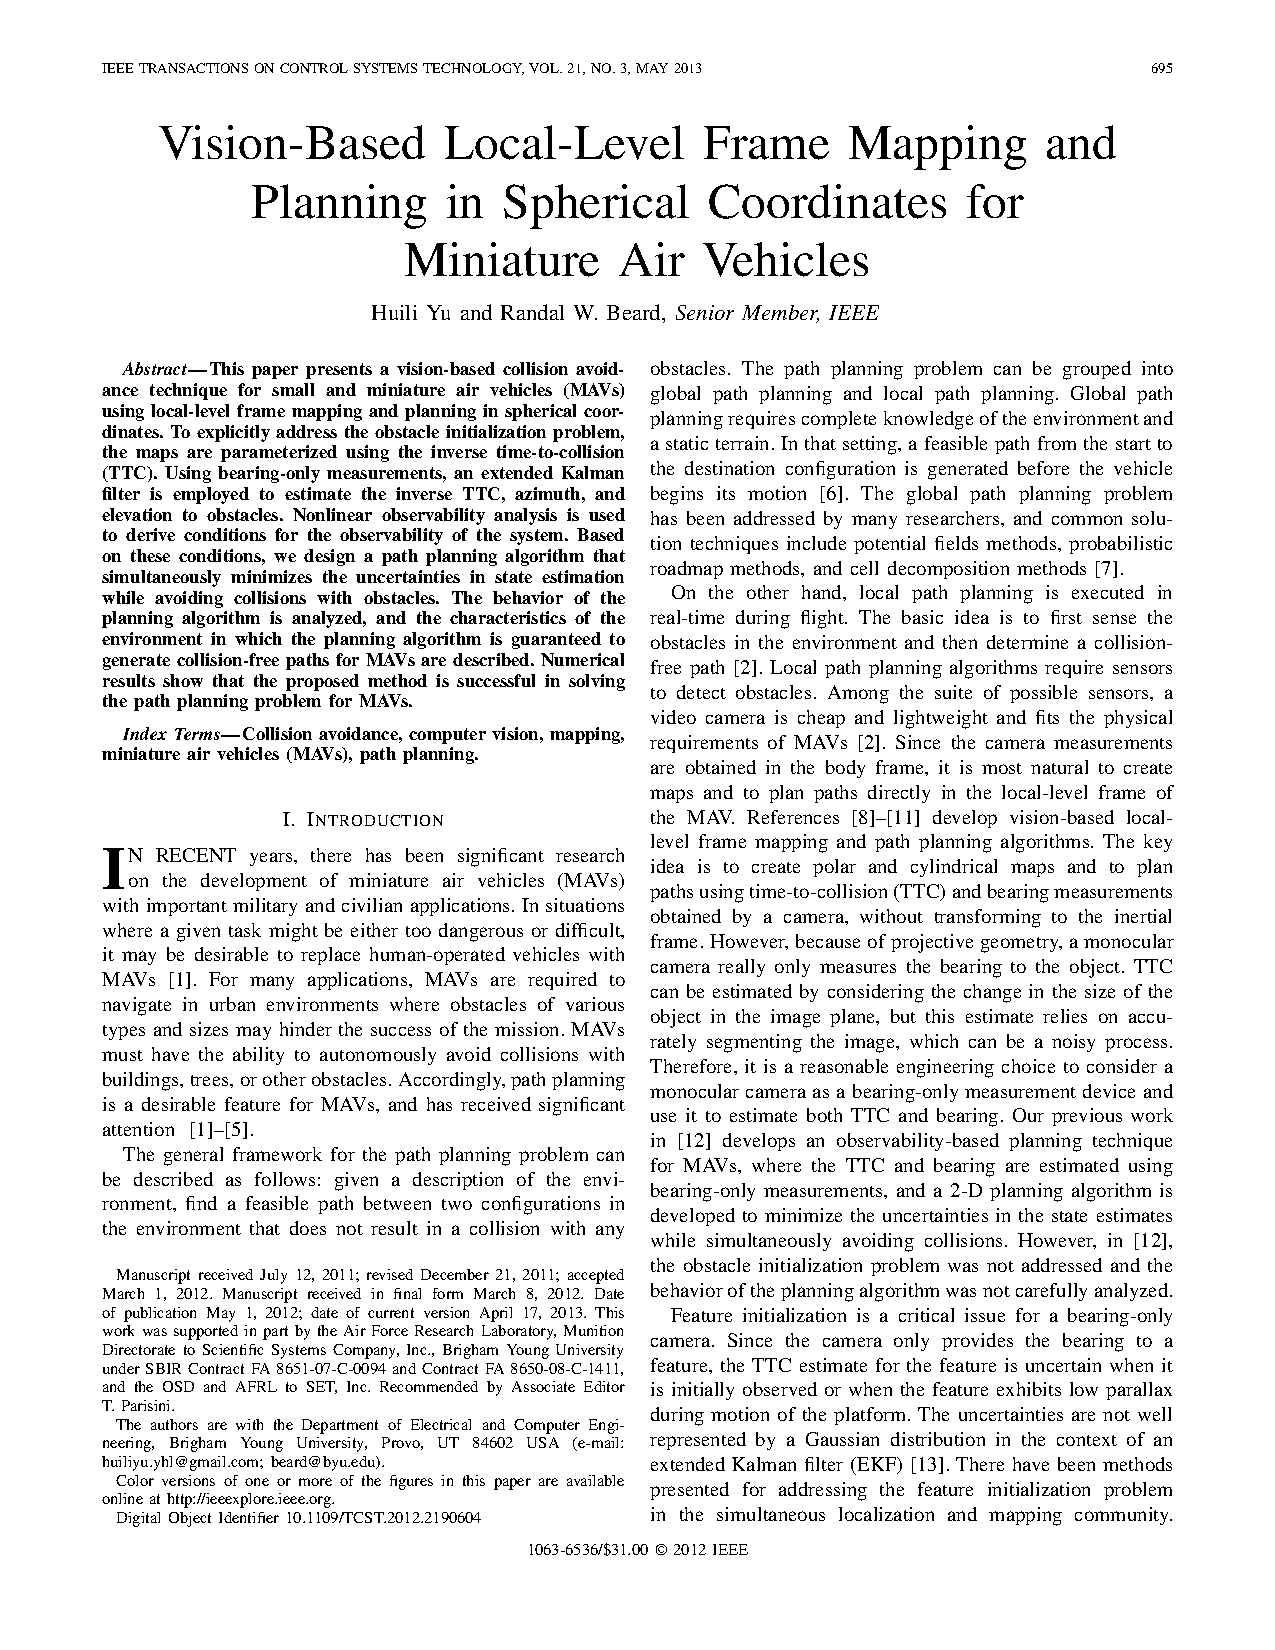
\includepdf[pages=-,scale=.8,pagecommand={}]{chap9_visual_servoing/papers/YuBeard13a.pdf}
%
%\section{Vision-Based UAV Collision Avoidance with 2D Dynamic Safety Envelop, AESM, 2016}
%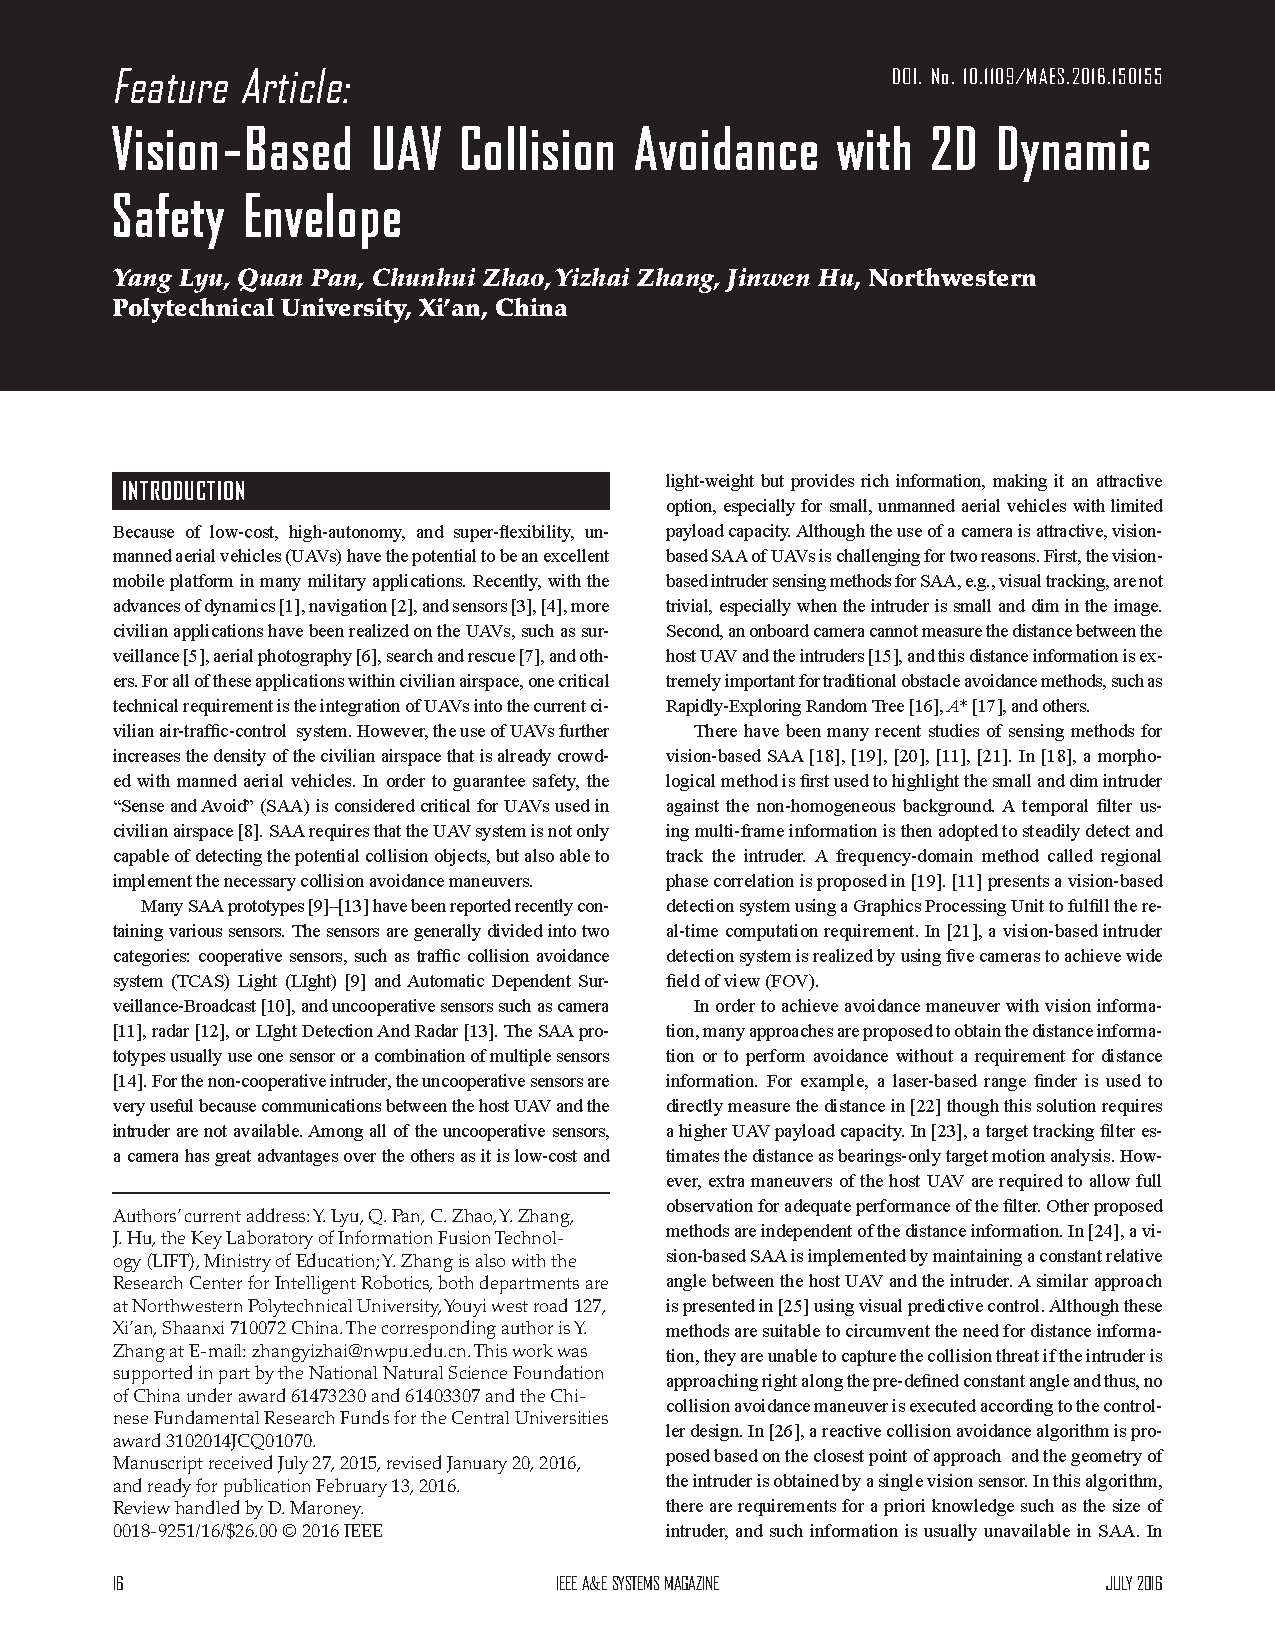
\includepdf[pages=-,scale=.8,pagecommand={}]{chap9_visual_servoing/papers/LyuPanZhao16.pdf}

